\documentclass[12pt,a4paper]{article}

\usepackage[utf8]{inputenc}
\usepackage[T1]{fontenc}
\usepackage{geometry}
\geometry{margin=1in}
\usepackage{graphicx}
\usepackage{booktabs}
\usepackage{amsmath}
\usepackage{pgfplots}
\pgfplotsset{compat=1.18}
\usepackage{hyperref}
\usepackage{listings}
\usepackage{xcolor}
\usepackage{float}
\usepackage{caption}
\usepackage{enumitem}
\usepackage{multicol}
\usepackage{fancyhdr}

\pagestyle{fancy}
\fancyhf{}
\rhead{Sabbir Ahmmed}
\lhead{AI Assignment 4}
\cfoot{\thepage}

\lstset{
  language=C++,
  basicstyle=\ttfamily\small,
  keywordstyle=\color{blue}\bfseries,
  commentstyle=\color{gray},
  stringstyle=\color{red},
  breaklines=true,
  frame=single,
  numbers=left,
  numberstyle=\tiny\color{gray},
}

\title{\textbf{AI Assignment 4}\\[0.3em]
\Large Travelling Salesman Problem (TSP)\\
Using Greedy Technique and Simulated Annealing}
\author{Sabbir Ahmmed\\Student ID: 2205040}
\date{September 7, 2026}

\begin{document}
\maketitle
\tableofcontents
\newpage

%==========================================================================
\section{Assignment Overview}
%==========================================================================

The Travelling Salesman Problem (TSP) is one of the most well-known NP-hard optimization problems in computer science. A salesman must visit a number of cities exactly once and return to the starting city, minimizing the total travelling cost.

This assignment implements two approaches:
\begin{enumerate}
    \item \textbf{Greedy Technique (Nearest Neighbor)} --- to quickly construct a feasible solution.
    \item \textbf{Simulated Annealing} --- a metaheuristic optimization technique designed to improve solutions and escape local optima.
\end{enumerate}

The goal is to implement, test, compare, and analyze both techniques across multiple TSP instances of varying sizes.

%==========================================================================
\section{Problem Description}
%==========================================================================

Given $N$ cities and a travelling cost between every pair of cities, the task is to find a tour that:
\begin{enumerate}
    \item Starts from a specified starting city (City 0).
    \item Visits every city exactly once.
    \item Returns to the starting city.
    \item Minimizes the total travelling cost.
\end{enumerate}

For a tour $0 \to c_1 \to c_2 \to \cdots \to c_{N-1} \to 0$, the total cost is:
\[
\text{Cost} = \sum_{i=0}^{N-1} \text{cost}(c_i, c_{(i+1) \bmod N})
\]

%==========================================================================
\section{Input Format}
%==========================================================================

The input is a text file with the following format:
\begin{verbatim}
N
c[0][0] c[0][1] c[0][2] ... c[0][N-1]
c[1][0] c[1][1] c[1][2] ... c[1][N-1]
...
c[N-1][0] c[N-1][1] ... c[N-1][N-1]
\end{verbatim}

\noindent Assumptions:
\begin{itemize}
    \item $2 \leq N \leq 500$
    \item $\text{cost}(i, i) = 0$
    \item All other costs are positive.
    \item The matrix may be symmetric or asymmetric.
    \item City numbering starts from 0.
\end{itemize}

%==========================================================================
\section{Implementation}
%==========================================================================

%--------------------------------------------------------------------------
\subsection{Greedy Algorithm (Nearest Neighbor)}
%--------------------------------------------------------------------------

The greedy heuristic builds a tour by always choosing the nearest unvisited city:

\begin{enumerate}
    \item Start at City 0. Mark it as visited.
    \item Among all unvisited cities, select the one with minimum travelling cost from the current city.
    \item Move to the selected city, mark it as visited.
    \item Repeat until all cities have been visited.
    \item Return to City 0.
\end{enumerate}

\textbf{Time Complexity:} $O(N^2)$ --- At each of the $N$ steps, we scan all $N$ cities to find the nearest unvisited one.

%--------------------------------------------------------------------------
\subsection{Simulated Annealing}
%--------------------------------------------------------------------------

Simulated Annealing is inspired by the physical process of annealing in metallurgy. A solution is iteratively improved by:

\begin{enumerate}
    \item \textbf{Initial Solution:} Either a random permutation or the greedy tour.
    \item \textbf{Neighbor Generation:} Using 2-opt segment reversal: pick positions $1 \leq i < j < N$, reverse the segment $[i, j]$.
    \item \textbf{Acceptance Rule:}
    \begin{itemize}
        \item If $\Delta \leq 0$ (improvement): always accept.
        \item If $\Delta > 0$ (worsening): accept with probability $P = e^{-\Delta/T}$.
    \end{itemize}
    \item \textbf{Cooling Schedule:} Geometric cooling $T_{k+1} = \alpha \cdot T_k$.
    \item \textbf{Termination:} When $T < T_{\min}$ or maximum iterations reached.
\end{enumerate}

\textbf{Time Complexity:} $O(I \cdot N)$ where $I$ is the total number of iterations. Each iteration generates a neighbor in $O(N)$ (segment reversal) and recalculates the tour cost in $O(N)$.

%--------------------------------------------------------------------------
\subsection{Key Implementation Details}
%--------------------------------------------------------------------------

The codebase is organized into the following modular components:

\begin{table}[H]
\centering
\caption{Implementation Functions}
\begin{tabular}{@{}ll@{}}
\toprule
\textbf{Function} & \textbf{Purpose} \\
\midrule
\texttt{readInput()} & Read cost matrix from file \\
\texttt{calculateTourCost()} & Compute total tour cost including return edge \\
\texttt{greedyTSP()} & Nearest Neighbor heuristic \\
\texttt{generateRandomTour()} & Random permutation with City 0 fixed \\
\texttt{generateNeighbor()} & 2-opt segment reversal \\
\texttt{simulatedAnnealing()} & Full SA algorithm with metrics \\
\texttt{printResults()} & Formatted output \\
\texttt{isValidTour()} & Tour validation \\
\texttt{generateEuclideanInstance()} & Random Euclidean cost matrix generator \\
\bottomrule
\end{tabular}
\end{table}

%==========================================================================
\section{Experimental Setup}
%==========================================================================

Five TSP instances of increasing size were generated using random Euclidean coordinates:

\begin{table}[H]
\centering
\caption{Test Instances}
\begin{tabular}{@{}lccc@{}}
\toprule
\textbf{Instance} & \textbf{Cities} & \textbf{Type} & \textbf{Seed} \\
\midrule
Test1\_10 & 10 & Euclidean & 1244 \\
Test2\_20 & 20 & Euclidean & 1254 \\
Test3\_50 & 50 & Euclidean & 1284 \\
Test4\_100 & 100 & Euclidean & 1334 \\
Test5\_200 & 200 & Euclidean & 1434 \\
\bottomrule
\end{tabular}
\end{table}

\noindent Default SA parameters: $T_0 = 1000$, $\alpha = 0.995$, $T_{\min} = 0.001$, iterations per temperature = 100, maximum iterations = 100{,}000.

%==========================================================================
\section{Experiment 1: Greedy vs. Simulated Annealing}
%==========================================================================

For each instance, the greedy algorithm was run once, and SA was run 5 times with different seeds. Results:

\begin{table}[H]
\centering
\caption{Experiment 1 Results}
\begin{tabular}{@{}lrrrrrr@{}}
\toprule
\textbf{Instance} & \textbf{Cities} & \textbf{Greedy} & \textbf{SA Best} & \textbf{SA Avg} & \textbf{Improve\%} & \textbf{Time(s)} \\
\midrule
Test1\_10 & 10 & 2462 & 2376 & 2376 & 3.49\% & 0.0098 \\
Test2\_20 & 20 & 4916 & 4170 & 4176 & 15.17\% & 0.0123 \\
Test3\_50 & 50 & 7387 & 5887 & 5985 & 20.31\% & 0.0235 \\
Test4\_100 & 100 & 10379 & 8315 & 8556 & 19.89\% & 0.0342 \\
Test5\_200 & 200 & 13521 & 13349 & 13624 & 1.27\% & 0.0592 \\
\bottomrule
\end{tabular}
\end{table}

\begin{figure}[H]
\centering
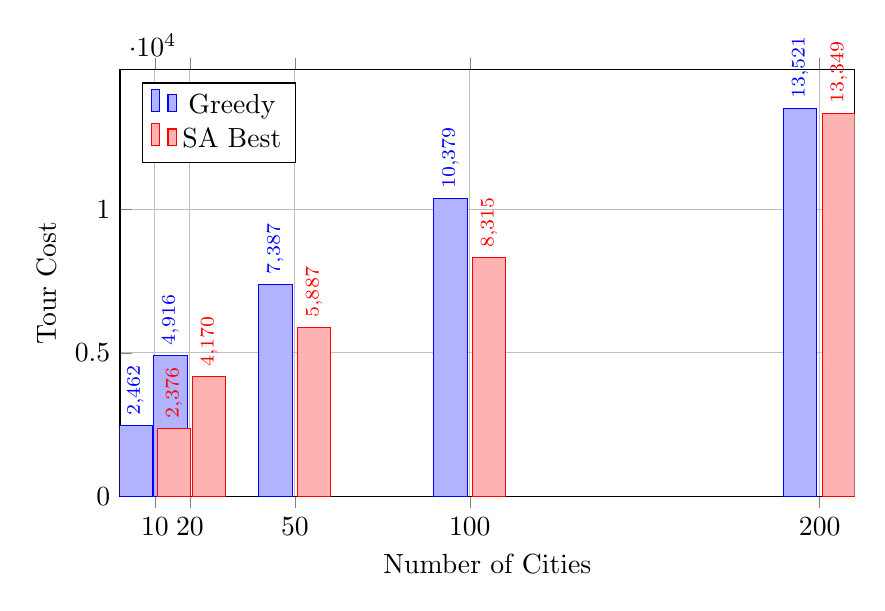
\begin{tikzpicture}
\begin{axis}[
    width=0.9\textwidth,
    height=7cm,
    ylabel={Tour Cost},
    xlabel={Number of Cities},
    legend pos=north west,
    grid=major,
    xtick={10,20,50,100,200},
    xmin=0, xmax=210,
    ymin=0,
    bar width=12pt,
    ybar,
    nodes near coords,
    every node near coord/.append style={font=\scriptsize, rotate=90, anchor=west},
]
\addplot coordinates {(10,2462) (20,4916) (50,7387) (100,10379) (200,13521)};
\addplot coordinates {(10,2376) (20,4170) (50,5887) (100,8315) (200,13349)};
\legend{Greedy, SA Best}
\end{axis}
\end{tikzpicture}
\caption{Greedy vs. SA Best Cost across instances}
\end{figure}

\begin{figure}[H]
\centering
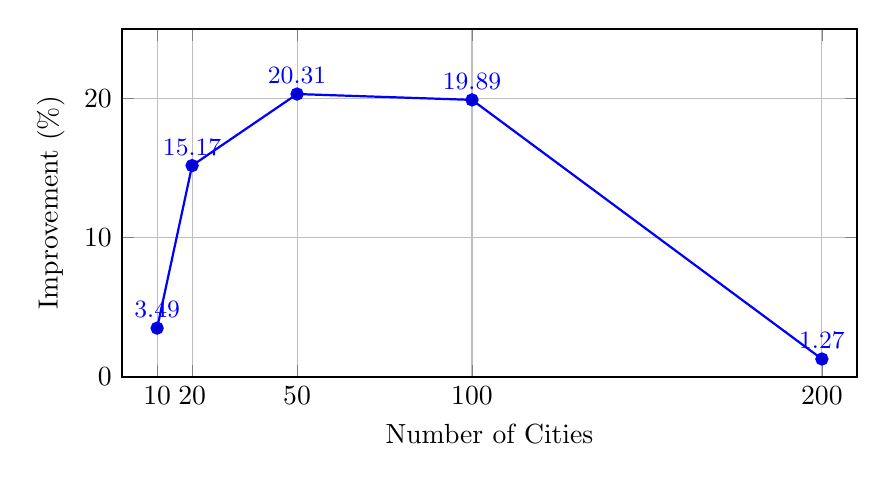
\begin{tikzpicture}
\begin{axis}[
    width=0.9\textwidth,
    height=6cm,
    ylabel={Improvement (\%)},
    xlabel={Number of Cities},
    grid=major,
    xtick={10,20,50,100,200},
    xmin=0, xmax=210,
    ymin=0, ymax=25,
    mark=*,
    thick,
    nodes near coords,
    every node near coord/.append style={font=\small, above},
]
\addplot coordinates {(10,3.49) (20,15.17) (50,20.31) (100,19.89) (200,1.27)};
\end{axis}
\end{tikzpicture}
\caption{SA improvement over Greedy (\%)}
\end{figure}

\paragraph{Discussion:}
SA consistently outperforms the greedy solution, with improvements ranging from 1.27\% to 20.31\%. The largest improvement is observed at $N=50$ (20.31\%). For the 200-city instance, the improvement is modest (1.27\%), likely because the fixed iteration budget (100{,}000) becomes insufficient for larger instances. The greedy algorithm runs in microseconds while SA takes tens of milliseconds, but the solution quality improvement justifies the extra computation.

%==========================================================================
\section{Experiment 2: Varying Initial Temperature ($T_0$)}
%==========================================================================

Using the 50-city instance with $T_0 \in \{100, 1000, 5000\}$:

\begin{table}[H]
\centering
\caption{Experiment 2 Results}
\begin{tabular}{@{}rrrrr@{}}
\toprule
\textbf{$T_0$} & \textbf{Best Cost} & \textbf{Accepted Moves} & \textbf{Worse Accepted} & \textbf{Time(s)} \\
\midrule
100 & 5977 & 3565 & 647 & 0.0205 \\
1000 & 5940 & 25976 & 11911 & 0.0197 \\
5000 & 6508 & 54705 & 26249 & 0.0201 \\
\bottomrule
\end{tabular}
\end{table}

\begin{figure}[H]
\centering
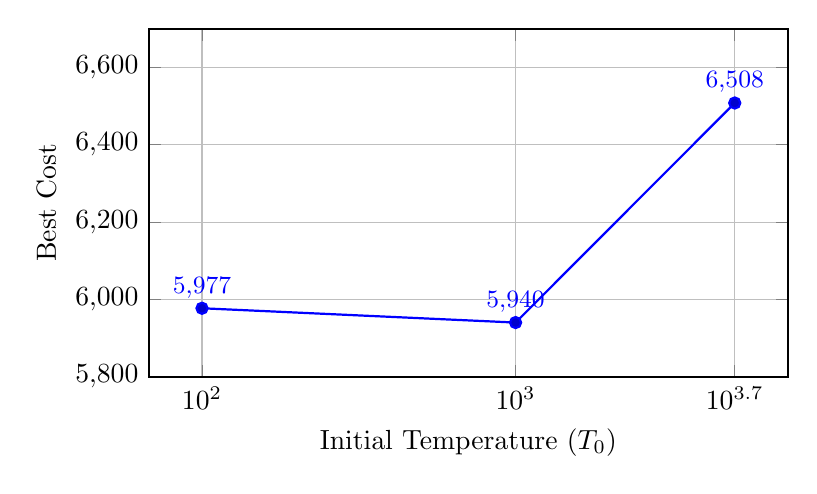
\begin{tikzpicture}
\begin{axis}[
    width=0.8\textwidth,
    height=6cm,
    ylabel={Best Cost},
    xlabel={Initial Temperature ($T_0$)},
    xtick={100,1000,5000},
    xmode=log,
    grid=major,
    mark=*,
    thick,
    nodes near coords,
    every node near coord/.append style={font=\small, above},
    ymin=5800, ymax=6700,
]
\addplot coordinates {(100,5977) (1000,5940) (5000,6508)};
\end{axis}
\end{tikzpicture}
\caption{Best cost vs.\ initial temperature}
\end{figure}

\paragraph{Discussion:}
\begin{itemize}
    \item \textbf{Low $T_0$ (100):} Accepts only 647 worse moves. The algorithm behaves like a greedy local search --- converges quickly but risks getting trapped in a local optimum (cost = 5977).
    \item \textbf{Moderate $T_0$ (1000):} Accepts 11{,}911 worse moves, achieving the best cost of 5940. This value balances exploration and exploitation within the iteration budget.
    \item \textbf{High $T_0$ (5000):} Accepts 26{,}249 worse moves --- too much exploration early on wastes iterations before the temperature drops enough for the search to converge. The final cost (6508) is worse than even the low-$T_0$ run.
\end{itemize}

%==========================================================================
\section{Experiment 3: Varying Cooling Rate ($\alpha$)}
%==========================================================================

Using the 50-city instance with $\alpha \in \{0.90, 0.95, 0.995\}$:

\begin{table}[H]
\centering
\caption{Experiment 3 Results}
\begin{tabular}{@{}rrrr@{}}
\toprule
\textbf{$\alpha$} & \textbf{Best Cost} & \textbf{Temp Steps to $T_{\min}$} & \textbf{Time(s)} \\
\midrule
0.900 & 6104 & 132 & 0.0026 \\
0.950 & 6117 & 270 & 0.0054 \\
0.995 & 5940 & 2757 & 0.0200 \\
\bottomrule
\end{tabular}
\end{table}

\begin{figure}[H]
\centering
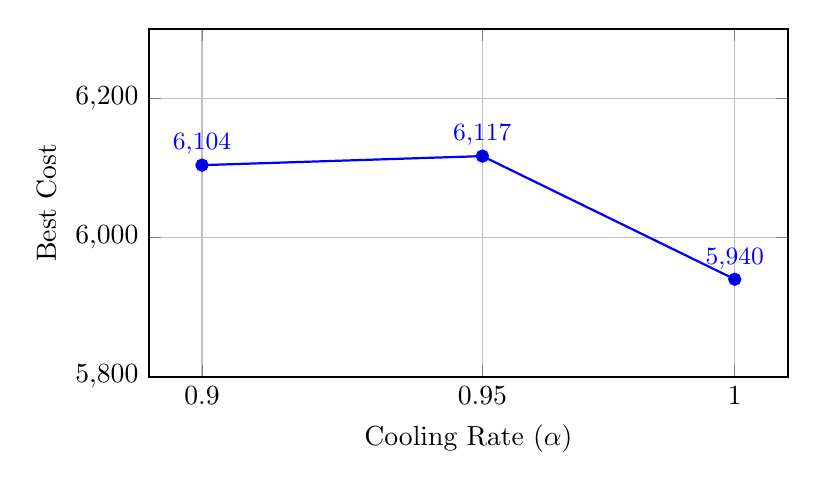
\begin{tikzpicture}
\begin{axis}[
    width=0.8\textwidth,
    height=6cm,
    ylabel={Best Cost},
    xlabel={Cooling Rate ($\alpha$)},
    xtick={0.90,0.95,0.995},
    grid=major,
    mark=*,
    thick,
    nodes near coords,
    every node near coord/.append style={font=\small, above},
    ymin=5800, ymax=6300,
]
\addplot coordinates {(0.90,6104) (0.95,6117) (0.995,5940)};
\end{axis}
\end{tikzpicture}
\caption{Best cost vs.\ cooling rate}
\end{figure}

\paragraph{Discussion:}
\begin{itemize}
    \item \textbf{Fast cooling ($\alpha = 0.90$):} Reaches $T_{\min}$ in only 132 temperature steps. The search spends very little time at each temperature and freezes quickly into a local optimum (cost = 6104). Computation is cheap (0.0026s).
    \item \textbf{Moderate cooling ($\alpha = 0.95$):} Takes 270 steps. Slightly worse than $\alpha = 0.90$ in this run (cost = 6117), likely due to random variation.
    \item \textbf{Slow cooling ($\alpha = 0.995$):} Takes 2{,}757 steps --- far more temperature levels. This gives the algorithm much more time to explore the solution space and escape local optima, achieving the best cost of 5940. The computational cost (0.02s) is still very manageable.
\end{itemize}

%==========================================================================
\section{Experiment 4: Random vs. Greedy Initialization}
%==========================================================================

Using the 50-city instance, SA was run 5 times with each initialization method:

\begin{table}[H]
\centering
\caption{Experiment 4 Results}
\begin{tabular}{@{}lrrrr@{}}
\toprule
\textbf{Init Method} & \textbf{Best} & \textbf{Avg} & \textbf{Worst} & \textbf{Avg Time(s)} \\
\midrule
Random & 5917 & 5974 & 6023 & 0.0196 \\
Greedy & 5981 & 6041 & 6207 & 0.0197 \\
\bottomrule
\end{tabular}
\end{table}

\begin{figure}[H]
\centering
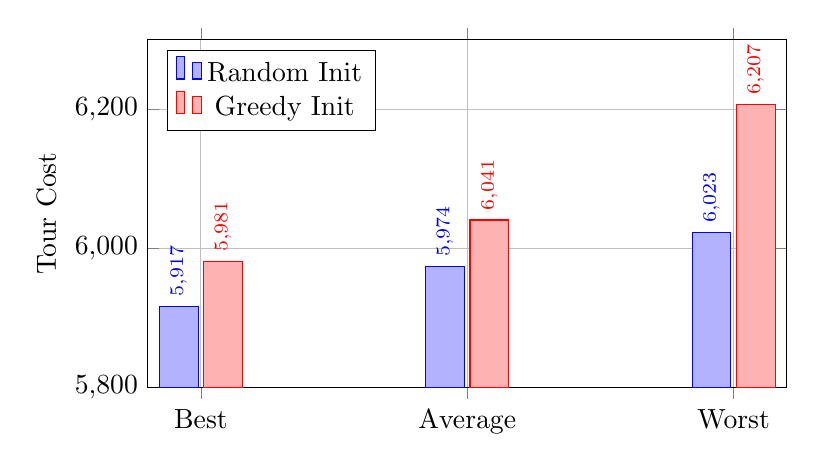
\begin{tikzpicture}
\begin{axis}[
    width=0.8\textwidth,
    height=6cm,
    ylabel={Tour Cost},
    xlabel={},
    xtick=data,
    xticklabels={Best, Average, Worst},
    legend pos=north west,
    grid=major,
    bar width=14pt,
    ybar,
    nodes near coords,
    every node near coord/.append style={font=\scriptsize, rotate=90, anchor=west},
    ymin=5800, ymax=6300,
]
\addplot coordinates {(1,5917) (2,5974) (3,6023)};
\addplot coordinates {(1,5981) (2,6041) (3,6207)};
\legend{Random Init, Greedy Init}
\end{axis}
\end{tikzpicture}
\caption{Random vs.\ Greedy initialization comparison}
\end{figure}

\paragraph{Discussion:}
In these runs, random initialization achieved better results than greedy initialization across all metrics (best, average, worst). This is because:
\begin{itemize}
    \item Random initialization provides diverse starting points, giving SA a better chance of exploring different basins of attraction in the solution space.
    \item Greedy initialization starts SA in a nearby region of the search space. With a limited iteration budget, SA may not have enough iterations to move far from the greedy starting point.
    \item For larger iteration budgets, greedy initialization would likely outperform random initialization because it starts closer to a good solution.
\end{itemize}

This result highlights an important practical consideration: the effectiveness of the initialization strategy depends on the interaction between the starting solution quality and the available computational budget.

%==========================================================================
\section{Complexity Analysis}
%==========================================================================

%--------------------------------------------------------------------------
\subsection{Greedy Technique}
%--------------------------------------------------------------------------

The Nearest Neighbor algorithm has time complexity $O(N^2)$:
\begin{itemize}
    \item At each of the $N$ steps, the algorithm scans all $N$ cities to find the nearest unvisited one.
    \item The tour cost calculation is $O(N)$.
    \item Overall: $O(N^2)$ for the tour construction, plus $O(N)$ for cost calculation.
\end{itemize}

Space complexity: $O(N^2)$ for the cost matrix.

%--------------------------------------------------------------------------
\subsection{Simulated Annealing}
%--------------------------------------------------------------------------

Let $I$ be the total number of iterations:
\begin{itemize}
    \item \textbf{Neighbor generation (2-opt reversal):} $O(N)$ per iteration.
    \item \textbf{Tour cost recalculation:} $O(N)$ per iteration (full recalculation).
    \item \textbf{Per-iteration cost:} $O(N)$.
    \item \textbf{Total time:} $O(I \cdot N)$.
\end{itemize}

\paragraph{Potential Optimization:} Instead of recalculating the entire tour cost after each 2-opt reversal, we can compute only the delta in $O(1)$:
\[
\Delta = \text{cost}(i-1, j) + \text{cost}(i, j+1) - \text{cost}(i-1, i) - \text{cost}(j, j+1)
\]
This would reduce the per-iteration cost from $O(N)$ to $O(1)$, yielding an overall complexity of $O(I)$ for the inner loop. However, the current implementation uses full recalculation for simplicity and correctness.

Space complexity: $O(N^2)$ for the cost matrix.

%==========================================================================
\section{Comparative Summary}
%==========================================================================

\begin{table}[H]
\centering
\caption{Algorithm Comparison}
\begin{tabular}{@{}lcc@{}}
\toprule
\textbf{Aspect} & \textbf{Greedy} & \textbf{Simulated Annealing} \\
\midrule
Time Complexity & $O(N^2)$ & $O(I \cdot N)$ \\
Solution Quality & Local optimum & Near-global optimum \\
Determinism & Deterministic & Probabilistic \\
Escapes Local Optima & No & Yes \\
Parameters & None & $T_0$, $\alpha$, $T_{\min}$, iterations \\
Typical Improvement & --- & 3--20\% over Greedy \\
\bottomrule
\end{tabular}
\end{table}

%==========================================================================
\section{Conclusion}
%==========================================================================

This assignment demonstrates the trade-offs between a deterministic greedy heuristic and a probabilistic metaheuristic for the TSP:

\begin{enumerate}
    \item The \textbf{Greedy algorithm} provides a fast $O(N^2)$ solution but gets trapped in local optima. It is useful as a baseline or as an initialization for more advanced methods.
    \item \textbf{Simulated Annealing} consistently finds better tours (3--20\% improvement) at the cost of more computation. Its ability to accept worse moves allows it to escape local optima.
    \item \textbf{Parameter sensitivity} is critical: moderate initial temperature ($T_0 = 1000$) and slow cooling ($\alpha = 0.995$) yield the best results for the tested instances.
    \item \textbf{Initialization strategy} interacts with the iteration budget: random initialization can outperform greedy initialization when the budget is limited, as it provides more diverse exploration.
\end{enumerate}

%==========================================================================
\section{Submission Contents}
%==========================================================================

\begin{itemize}
    \item \texttt{tsp2.cpp} --- Complete C++ source code
    \item \texttt{report.tex} --- This LaTeX report
    \item \texttt{report.txt} --- Raw experimental output
    \item \texttt{Test1\_10.txt} through \texttt{Test5\_200.txt} --- Generated test instances
\end{itemize}

\end{document}
